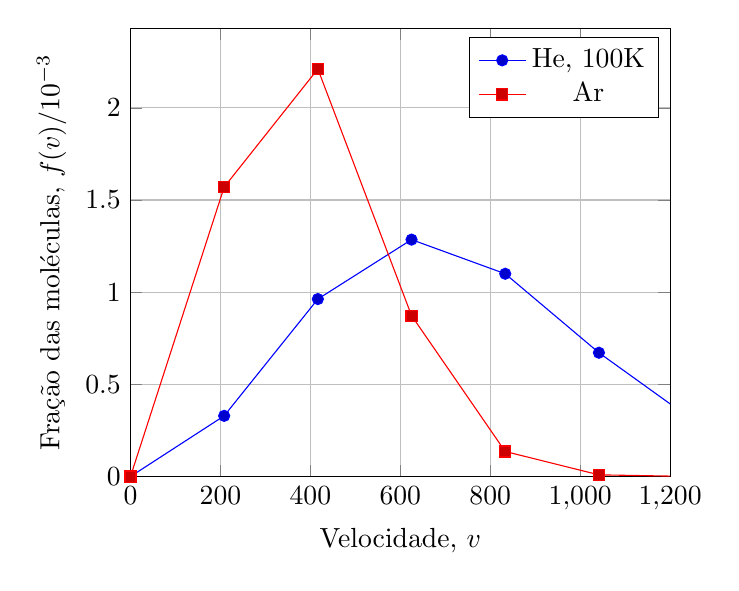
\begin{tikzpicture}
    \def\R{1000*8.314}% boltzmann constant
    \begin{axis}
        [
            grid = major,
            domain = 0:5000,
            xlabel = {Velocidade, $v$},
            ylabel = {Fração das moléculas, $f(v)/10^{-3}$},
            %xtick=\empty, 
            %ytick=\empty,
            xmin=0, ymin=0,
            xmax=1200,
        ]
    \pgfplotsinvokeforeach{4/100, 40/300} % razão M/T
    {
        \addplot
        {
            1000*sqrt(2/pi)*(#1/(\R))^(3/2)*x^2*exp(-#1/(\R)*x^2/2)
        };
    }
    \legend{{\ce{He}, \qty{100}{K}},\ce{Ar}}
\end{axis}
\end{tikzpicture}